\documentclass[11pt, a4paper]{report}
\usepackage[utf8]{inputenc}
\usepackage{amsmath, amsthm, amssymb, amsfonts, tikz, graphicx, listingsutf8, setspace, float}
\usepackage[obeyspaces]{url}
\usepackage[]{algorithm}
\usepackage{algpseudocode}[noend]
\usepackage{booktabs}
\usepackage{csvsimple}
\usepackage{multirow}

\definecolor{Code}{rgb}{0,0,0}
\definecolor{Decorators}{rgb}{0.4,0.0,0.4}
\definecolor{Numbers}{rgb}{0.5,0,0}
\definecolor{MatchingBrackets}{rgb}{0.25,0.5,0.5}
\definecolor{Keywords}{rgb}{0,0,1}
\definecolor{MoreKeys}{rgb}{0.8,0.05,0.1}
\definecolor{self}{rgb}{0,0,0}
\definecolor{Strings}{rgb}{0,0.63,0}
\definecolor{Comments}{rgb}{0,0.63,1}
\definecolor{Backquotes}{rgb}{0,0,0}
\definecolor{Classname}{rgb}{0,0,0}
\definecolor{FunctionName}{rgb}{0,0,0}
\definecolor{Operators}{rgb}{0,0,0}
\definecolor{Background}{rgb}{0.98,0.98,0.97}
\lstdefinelanguage{Python}{
numbers=left,
numberstyle=\footnotesize,
numbersep=1em,
xleftmargin=1em,
framextopmargin=2em,
framexbottommargin=2em,
showspaces=false,
showtabs=false,
showstringspaces=false,
frame=l,
tabsize=4,
% Basic
basicstyle=\ttfamily\small\setstretch{1},
backgroundcolor=\color{Background},
% Comments
commentstyle=\color{Comments}\slshape,
% Strings
stringstyle=\color{Strings},
morecomment=[s][\color{Strings}]{"""}{"""},,
morecomment=[s][\color{Strings}]{'''}{'''},
% keywords
morekeywords={class,def,while,format,range,if,is,elif,else,not,and,or,print,break,continue,return,True,False,None,access,as,del,except,exec,finally,global,lambda,pass,print,sum,raise,try,assert,linspace,array,abs,plot,append,gca,set_yscale,ylabel,xlabel,legend,axis,sin,cos,savefig,show,zip,binomial},
keywordstyle={\color{Keywords}\bfseries},
% additional keywords
morekeywords={[2]@invariant,pylab,plt,math,numpy,sympy,sp,matplotlib,pyplot,np,scipy},
keywordstyle={[2]\color{Decorators}\slshape},
emph={self},
emphstyle={\color{self}\slshape},
% keywords
morekeywords={[3],in,from,import,+,-,=,>,<,<=,>=,+=,-=},
keywordstyle={[3]\color{MoreKeys}\bfseries},
%
}

\lstset{
    inputencoding=utf8/latin1,
    breaklines=true
}

\newcommand*\Heq{\ensuremath{\overset{\kern2pt L'H}{=}}}

\newcommand{\tvect}[2]{%
    \ensuremath{\Bigl(\negthinspace\begin{smallmatrix}#1\\#2\end{smallmatrix}\Bigr)
}}

\setlength\parindent{0pt}
\linespread{1.3}
\lstset{language=Python}

\csvstyle{optimalModel}{tabular=|l | l | c | c | c | c |,
    table head=Model & Technique & $\lambda$ & Poly & Validation MSE & Test MSE}

\setlength{\parskip}{.6em}

\title{FYS-STK3155 Project 1}
\author{Didrik Sten Ingebrigtsen}
\date{\today}

\begin{document}

\maketitle

\chapter{Abstract}

Linear regression is an easy and highly interpretable form of machine learning. It does however still require some tuning, that quickly becomes less intuitive once the dimensionality and/or the complexity of the data rises. In this report we will describe a process for tuning by splitting the data into three sets, and using resampling methods to estimate how well different hyperparameters perform using only two of them. Lastly, we discuss how well this tuning process is at finding the best models, by testing it on the third set.

\chapter{Introduction}

The main objective of this project was to implement code for simple and regularised linear regression methods, and to find optimal hyperparameters and their associated errors for both the Franke function and actual terrain data. To do this, the question of how to measure what is optimal is key, and within that lies an important discussion of bias and variance.

To solve this problem, we have firstly implemented bootstrap and k-fold resampling techinques, and tested their capabilities on the predictable and flexible Franke function. After the next section, where we describe linear regression more precisely, is a section on this validation of my implementation and techniques. Then, we apply this to actual terrain data, and tune our hyperparameters. Lastly, we discuss the results, and further implications on linear regression and hyperparameter optimalisation.

\chapter{Theory}

\section{Linear regression}

Linear regression is a class of regression where the predictor variable is taken through some set of functions to make a design matrix $X$ where each row represents a datapoint and each column a function.\footnote[1]{This, as well asthe other theory, is adapted from Hjorth-Jensen(2020) and Hastie et. al (2009)} Then, a vector of parameters $\beta$ is multiplied to it, and a regularisation term $\lambda R$ (where $\lambda$ is the regularisation coefficient) that could be a function of both the design matrix and the parameters could also be subtracted. Since I am working with terrain, and for simplicities sake, I have limited myself to these functions going into the design matrix being a basis expansion (making the columns of $X$ polynomial). To sum up, this is my model:

\[ \tilde{y} = X \beta - \lambda R \]

In here, each columns of an n-dimensional $X$ is on the form $x_0^{p_0} \cdot x_1^{p_1} \cdot ... \cdot x_{n-1}^{p_{n-1}}$ for all $p$ that satisfies the condition $\sum_{i=0}^n p_i \leq P$ where $P$ is the maximum polynomial, a hyperparameter.

The assumptions needed for linear regression with the design matrix made with these polynomials is that our dependent variable is composed of some underlying polynomial function and an error term:

\[ y = f(x) + \varepsilon \]

\section{Fitting and overfitting}

To make a concrete model, we have to fit a $\beta$ to our $X$ and $y$ data. This is done by defining some cost function, a function taking in our model and some data and our model and returning error, and minimizing this function. The by far most common cost function, at least for linear regression, is the residual sum of squares ($RSS$). This is the sum of the squared differences from our prediction and our actual data. Minimizing this is the same as finding the points where the first order partial derivative is 0, and the second order partial derivative is positive, both with regards to $\beta$

\begin{align}
RSS &= (y - X \beta)^T (y - X \beta) \\
\frac{\partial RSS}{\partial{\beta}} &= -2 X^T (y - X \beta) \\
\frac{\partial^2 RSS}{\partial \beta \partial \beta^T} &= 2 X^T X
\end{align}

Given that X is invertible (which we'll come back to later), $\frac{\partial^2 RSS}{\partial \beta \partial \beta^T} > 0$,and so any value of $\beta$ that satisfies $\frac{\partial RSS}{\partial{\beta}}=0$, is an optimal $\beta$, or a $\hat{\beta}$.

\begin{align}
\frac{\partial RSS}{\partial{\beta}} &= -2 X^T (y - X \beta) \\
0 &= X^T (y - X \beta) \\
\hat{\beta} &= (X^T X)^{-1} X^T y
\end{align}

If our dependent variable was just a polynomial of a manageably low degree, this would be enough. However, because of our noise term $\varepsilon$, minimizing $RSS$ doesn't just fit our $\hat{\beta}$ to the actual underlying structure. Therefore, the $RSS$ score found for $\hat{\beta}$ isn't a good estimate of how good our model would do to for any new data. To see how good a model is, we therefore split the data into several parts, at least a training and testing set. Training data is used to find some $\hat{\beta}$, and the testing data is held back until we want to evaluate the model. If we want to select hyperparameters like $P$ and $\lambda$, we should also evaluate our model on some dataset that isn't the training set, but also not the testing set, so that we get an honest evaluation of how good the model is on unseen data in the end, and don't tailor neither the parameters or the hyperparameters to the testing data. That ss called overfitting, and would give us an inflated belief in our own model.

\section{Regularisation}

Another way to prevent overfitting, other than to split the data smartly, is to regularise it. Regularising is giving large parameter values some penalty. This prevents overfitting because parameters that have little predictive value in the training set, are highly unstable. If it turns out that this parameter has some higher importance in another dataset, then a large parameter value could make the estimate of the dependent variable explode. It's better for it to be small, and to therefore miss a potential structure, than to have it large and be likely to mistake small noise for an actual structure.

The two ways of regularisation we'll be looking at in this project is lasso and ridge regularisation. Both penalise high values for parameters, but their functions for determining how much to punish them is slightly different. Lasso subtracts the $L1$ distance, while ridge subtracts the $L2$ distance.

\section{Resampling}

When evaluating the model, and especially when data is scarce, it is very useful to resample. Resampling is a class of methods where you use your data more than one time, in different configurations, to see how different your model and errors could be given some hyperparameters. Conceptually, a high variance between errors estimated when evaluating a model trained on different samples of your data would indicate that the model is overfitting to the sampled data. Contrary, a low variance could indicate that the search for features isn't too aggressive, and could actually possibly be more aggressive. You can fit a bit more to the data. The consistent errors the models trained on the different samples make is called bias. These two values, the bias and the variance, often have a trade-off. A low variance often gives high bias, and vice versa. Resampling techniques can help find a good trade-off between them.

In this project, we will be using two common resampling techniques, bootstrap and k-fold. Bootstrap works by keeping a constant testing or validation set, and then selecting as many values as there are in the training set from it with replacement, and doing this many times. K-fold on the other hand mixes up training and testing or validation data into one set first, and then divides it into $k$ different sets. Then, one by one, each so-called fold is used as testing or validation data, while the others are used to train on.

To study the relationship between bias and variance, we will be using bootstrap resampling and looking at the variation and bias of the samples different predictions for each datapoint. The formulas needed to do this can be derived from the expectation value of mean squared error like this.

\begin{align}
E[MSE] &= E\left[(\pmb{y} - \pmb{\tilde{y}})^2 \right] = E\left[(\pmb{f} + \pmb{\epsilon} - \pmb{\tilde{y}})^2 \right] \\
&= E\left[(\pmb{f} + \pmb{\epsilon} - \pmb{\tilde{y}} + E[\pmb{\tilde{y}}] - E[\pmb{\tilde{y}}] )^2 \right] \\
&= E\left[\left(\pmb{f} - E[\pmb{\tilde{y}}\right)^2 \right] + E\left[\left(\pmb{\tilde{y}} - E[\pmb{\tilde{y}}\right)^2 \right] + E\left[\epsilon^2\right] \\
&+ E\left[2\pmb{f}\epsilon - 2\epsilon E[\pmb{\tilde{y}}]\right] + E\left[ 2\epsilon E[\pmb{\tilde{y}}] - 2\epsilon\pmb{\tilde{y}} \right] \\
&+ E\left[ 2\pmb{f} E[\pmb{\tilde{y}}] - 2E[\pmb{\tilde{y}}] - 2 \pmb{f} \pmb{\tilde{y}} + 2\pmb{\tilde{y}} E[\pmb{\tilde{y}}] \right] \\
&= E\left[ \left( \pmb{f} - E[\pmb{\tilde{y}}] \right)^2 \right] + E\left[ \left( \pmb{\tilde{y}} - E[\pmb{\tilde{y}}] \right)^2 \right] + \sigma^2 + 2\left( \pmb{f} - E[\pmb{\tilde{y}}] \right) \left( E[\pmb{\tilde{y}} - E[\pmb{\tilde{y}}\right) \\
&= E\left[ \left( \pmb{f} - E[\pmb{\tilde{y}}] \right)^2 \right] + E\left[ \left( \pmb{\tilde{y}} - E[\pmb{\tilde{y}}] \right)^2 \right] + \sigma^2
\end{align}

Here, the first term is the bias and the second the variation of our model, and the third the variance of the data noise. The bias term is like an integrative term that does something similar to summing up the errors, giving more weight to big ones than small ones. If it is high, there is some consistent error. The variance term doesn't relate to the real data at all, but only looks at how different each prediction of the same datapoint is, while the noise term is both hard to estimate, and hard to do anything with once the data is collected.

\chapter{Implementation}

\section{Data}
Our end goal is to make robust code that can handle real terrain data, and make a polynomial that fits well to it. Stated another way, we want to be able to make a function that takes in a coordinate, and returns height. To do this, let's start by considering how terrain data looks, and how it relates to polynomials.

Terrain is not smooth. If you were to get terrain data of infinite resolution, you would have to have a polynomial of infinite degrees to describe it perfectly. Since we have no ambition of being able to make some general claim about the nature of terrain, or apply our fitted model to anywhere but the exact area we have trained on, overfitting might not seem like a big risk. Any higher degree of complexity might seem as if it just describes our terrain more detailed. However, since we don't have continous data with infinite resolution, but only discrete samples, a polynomial of very high degree, fitted to this data, does run the risk of only being correct at our samples, and being very unpredictable in between them. This therefore seems like a great candidate for regularized linear regression. We optimally want to have a polynomial of high degree, but we want to penalize large parameters that might be unstable.

To establish a procedure for doing this, and verifying that it works, we will be using the Franke function, and an added noise term. This is flexible, because we can test different values for noise to see how well it generalises, and we also know exactly how the underlying structure is. The Franke function looks like this in writing

\begin{align*}
f(x_0, x_1) &= \frac{3}{4}\exp{\left(-\frac{(9x_0-2)^2}{4} - \frac{(9x_1-2)^2}{4}\right)}+\frac{3}{4}\exp{\left(-\frac{(9x_0+1)^2}{49}- \frac{(9x_1+1)}{10}\right)} \\
&+\frac{1}{2}\exp{\left(-\frac{(9x_0-7)^2}{4} - \frac{(9x_1-3)^2}{4}\right)} -\frac{1}{5}\exp{\left(-(9x_0-4)^2 - (9x_1-7)^2\right) }.
\end{align*}

, and plotted out in a square with $x_1, x_2 \in [-0.9, 1.1]$ it looks like \emph{fig \ref{fig:franke}}.

\begin{figure}
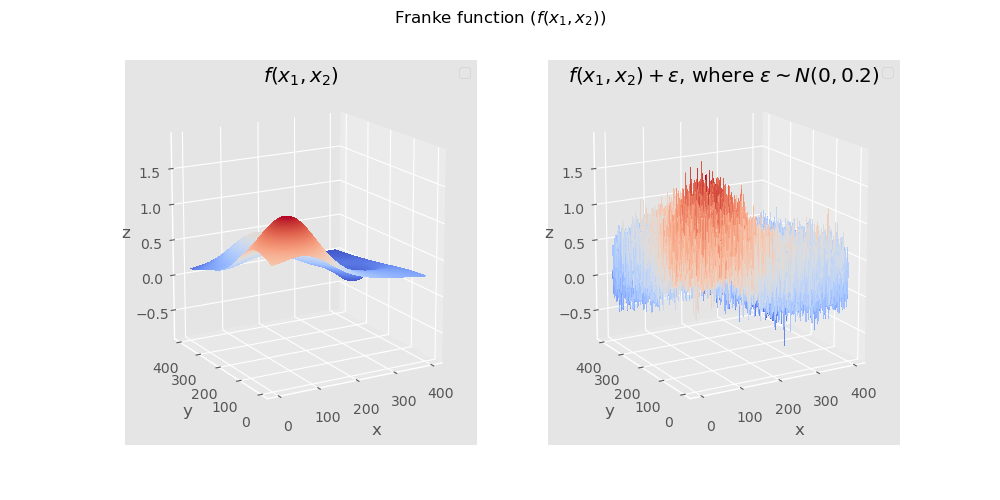
\includegraphics[width=\textwidth]{../plots/franke.png}
\caption{Franke function ($f(x_1, x_2)$) data, with the left being just $f(x_1, x_2)$ and the right being $f(x_1, x_2) + \varepsilon$, where $\varepsilon \sim N(0,0.2)$. The right one is the one being used as data.}
\label{fig:franke}
\end{figure}

\begin{figure}
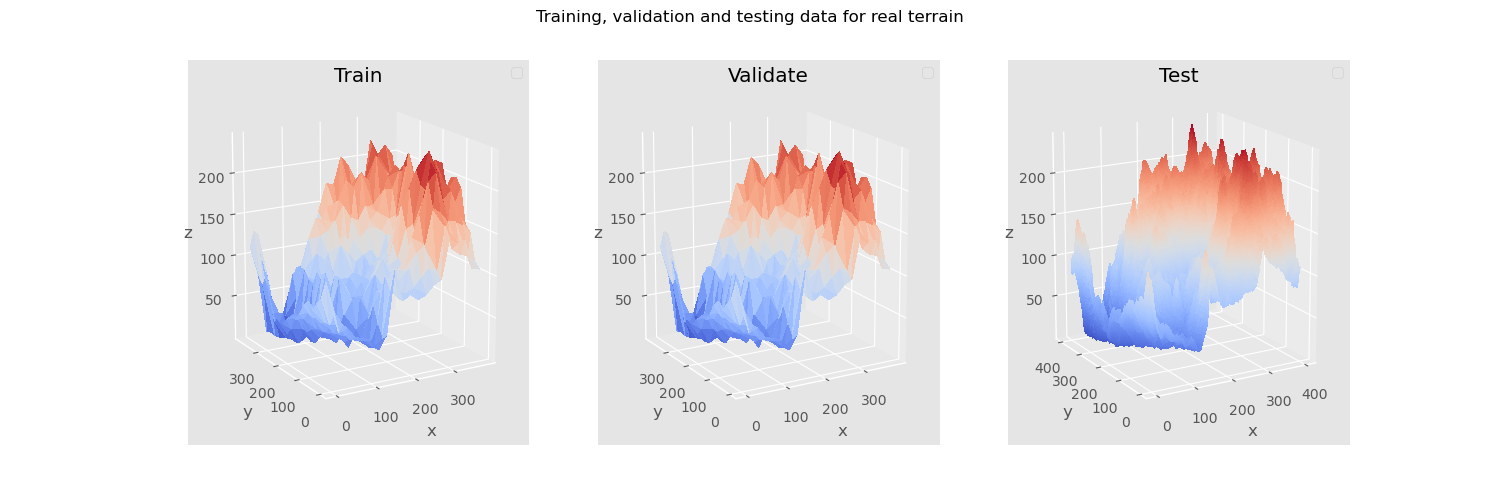
\includegraphics[width=\textwidth]{../plots/real_terrain.png}
\caption{The actual terrain we want to try out our methods on in the end, with one plot for each of our datasets.}
\label{fig:real_terrain}
\end{figure}

To handle this data, we need to split it into a training, validation and test set. Usually, choosing which parts of a dataset are put into these subsets is done at random or semi-random. The main reason for doing this is to prevent data bias. However, because our predictor variable is two dimensional and very easily interpretable, we argue that selecting training data on a grid ensures a low bias better than selecting randomly would. This gives an even distribution of points, and makes it so that there are no areas with low data coverage. The one potential bias this gives is for structures appearing in a grid themselves, but we have no reason to believe these are prevalent in terrain data.

There is another problem with this selection of data however, namely flexibility. Where as a random split grants fine tuned control of how large each subset should be, while as this grid gap parameter $x_sparsity$ is very course. This could be improved by making a more advanced function that selects a specific amount for training and validation per grid area, but we have not prioritised this.

\begin{figure}
\begin{center}
\caption{Portion of total data that is divided into the training, validation and testing sets respectively for different values of $x_{sparsity}$.}
\begin{tabular}{| c | c | c | c |}
\hline
$x_{sparsity}$ & \textbf{Training} & \textbf{Validation} & \textbf{Testing} \\
\hline
$1$ & $1$ & $0$ & $0$ \\
\hline
$2$ & $1/4$ & $1/4$ & $1/2$ \\
\hline
$3$ & $1/9$ & $1/9$ & $7/9$ \\
\hline
$4$ & $1/16$ & $1/16$ & $7/8$ \\
\hline
$5$ & $1/25$ & $1/25$ & $23/25$ \\
\hline
$10$ & $1/100$ & $1/100$ & $98/100$ \\
\hline
$20$ & $1/400$ & $1/400$ & $398/400$ \\
\hline
\end{tabular}
\label{table:xsparsity}
\end{center}
\end{figure}

Implementing this strategy is done in three steps:
\begin{enumerate}
    \item Select training set from a grid with some gap $x_{sparsity}$
    \item Select validation set from a grid with the same gap, but offset so that these points come in the middle between the training set datapoints
    \item Use the rest of the data as a testing set
\end{enumerate}

Files used for data creation and storing are \path{/python/data_handling.py}, \path{/python/franke.py} and \path{/python/real_terrain.py}, with \path{/python/test_data_handling.py} for testing.

\section{Models and training}

To implement the models, we made two classes, one for ordinary linear regression, and one for regularized versions, with the latter inheriting the predict-function from the first, and taking in a function for beta. The classes are quite simple, with the two main methods being fit and predict.

The files used for the models classes is \path{/python/linear_models.py} and \path{/python/test_linear_models.py}.

\section{Resampling}

To resample, we have implemented two functions; one for bootstrap and one for kfold cross-validation.

The bootstrap function is not vectorised, and works by making an array of equal length to $X_{train}$, but with random indeces from them, and then using those indeces to sample $X_{train}$ and $y_{train}$.

\lstinputlisting[language=Python,firstline=35,lastline=37]{../python/resampling.py}

Our kfold cross-validation algorithm is also very simple. However, it starts by selecting the data it will use in its folds from the training and validation datasets, and selects only as much data as it needs to make the total size of the training folds equalto the size of the original training set. This was in an attempt to make it and bootstrap perform more similarly, to get MSEs of the same scale, but was not very successful. Likely because bootstrap on picks only a subset of the training set every time, its MSE is consistently higher. The variance of our kfold techniques MSE estimate also seems heightened by picking a different set to train and validate everytime, but we also expect its bias to go down because any possible data bias is lowered due to it ot using the same data every time.

The file used for resampling is \path{/python/resampling.py}.

\section{Visualisation}

For visualisation, we have made two functions. One for plotting $n$ 3-dimensional plots in a grid, and the other for making different kinds of plots showing the relations between validation errors, maximum polynomial degree, and $\lambda$.

The first one is mainly useful for comparing predicted and actual terrain visually, and in addition to creating still images it can also make an animation spinning the plot around.

The second one is used for understanding the rich validation errors better, and understand what hyperparameters works best. It can make three different kinds of plots:
\begin{enumerate}
    \item An animation with lineplots showing the bootstrap estimated bias, variance and MSE of a model against $\lambda$, and with different maximum polynomials as time.
    \item An animation with lineplots showing the bootstrap estimated MSE and kfold estimated MSE of a model against $\lambda$, with different maximum polynomials as time
    \item Two still grid plots with $\lambda$ against polynomials, one for kfold estimated MSE, and one for bootstrap estimated MSE.
\end{enumerate}

The file used for visualisation is \path{/python/plotting.py}.

\section{Validating, tuning and testing}

In order to make our design matrixes we have a function that we think works particularly well. Because we want to emphasize hyperparameter optimalisation, but don't have access to any computing power other than the one our laptops can give us, we need to make efficient functions. The creation of a new design matrix is done once for every polynomial, and it's expensive for both large datasets and high maximum polynomials. To make an efficient function, we vectorised it, mitigated unnecessary recomputations, and in the process got very close to making it work for arbitrary input dimensions.

\begin{algorithm}
\caption{Pseudocode for polynomial design matrix function}
\begin{algorithmic}[0]
\Procedure{design matrix}{maxDegree, x}
    \State $powerCombinations \gets \{(p_1, p_2)\, |\, p_1 + p_2 \leq maxDegree \land p_1, p_2 \geq 0\}$
    \State $xPowers \gets \{(x^p)\, |\, p \leq maxDegree \land p \geq 0\}$
    \For{$(p_1, p_2) \in powerCombinations, n$}
        \State $X_n \gets xPowers^{p_1} \cdot xPowers^{p_2}$
    \EndFor
    \State \textbf{return} $X$
\EndProcedure
\end{algorithmic}
\end{algorithm}

The arguably most important part of this project is the tuning class, which iterates through different hyperparameters, uses the resampling techniques to estimate our error well, and stores all the data. It also computes optimal parameters as decided by the different resampling techniques, and tests it on the plentiful test data. The results this class produces, as well as the class itself and ways to improve it, is the main focus of the results and conclusion parts.

\chapter{Verifying our implementation on the Franke function}

Before we apply our methods to real terrain data, let's verify that it works as intended on the Franke function data. The code for this is in \path{/python/franke_verifying.py}.

\section{Small dataset}

Firstly, we want to check that we can induce overfitting, by using a small dataset, and allowing some complexity. In fig \ref{fig:franke_overfitting} it is easy to see that the model continues fit better to the training set for higher complexity, but quickly starts overfitting, and doing worse on the test set. The model actually does slightly better on the test set than the training set for low polynomial degrees, but this is just a coincidence that isn't that unlikely since the sets are so small.

\begin{figure}
\begin{center}
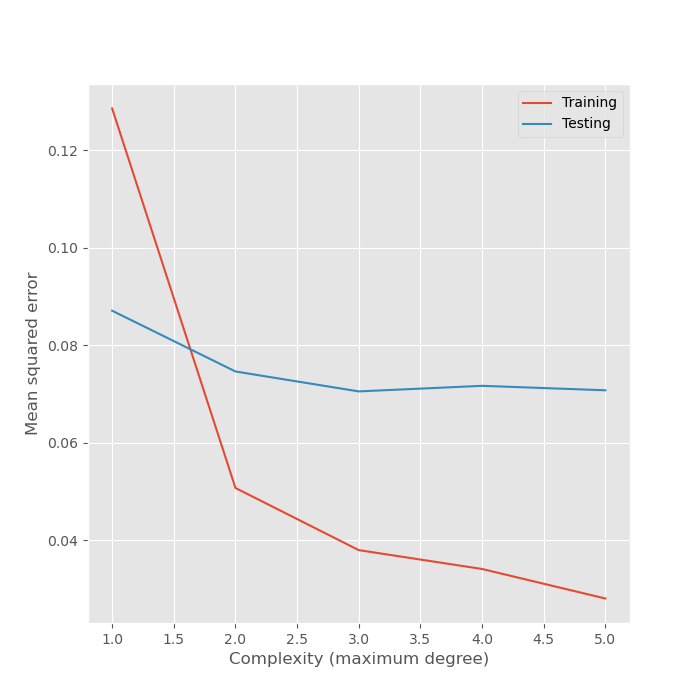
\includegraphics[width=0.5\textwidth]{../plots/overfitting_franke.png}
\end{center}
\caption{OLS models trained on only 49 datapoints, and tested on twice as much. Data from Franke function with noise.}
\label{fig:franke_overfitting}
\end{figure}

\section{$\beta$ parameters}

Next, we want to look at the $\beta$ parameters made by the last model whose error is plotted above, namely OLS with $p = 5$. It has $21$ parameters, and their standard deviation $\sigma$ can be computed by $\sigma_{\beta} = \sigma_y^2 (X^T X)^{-1}$, where $\sigma_y^2$ is the variance of the noise in $y$. This can be estimated by the mean squared error of $y$. It's not a good estimator, not even unbiased, but for this all we need is a rough idea of $\sigma_\beta^2$. Combining this, we can get the confidence intervals by assuming a normal distribution of $\beta$ values. In fig \ref{fig:conf_interval} we have plotted the interval for the different $\beta$ parameters with $99\%$ confidence.

\begin{figure}
\begin{center}
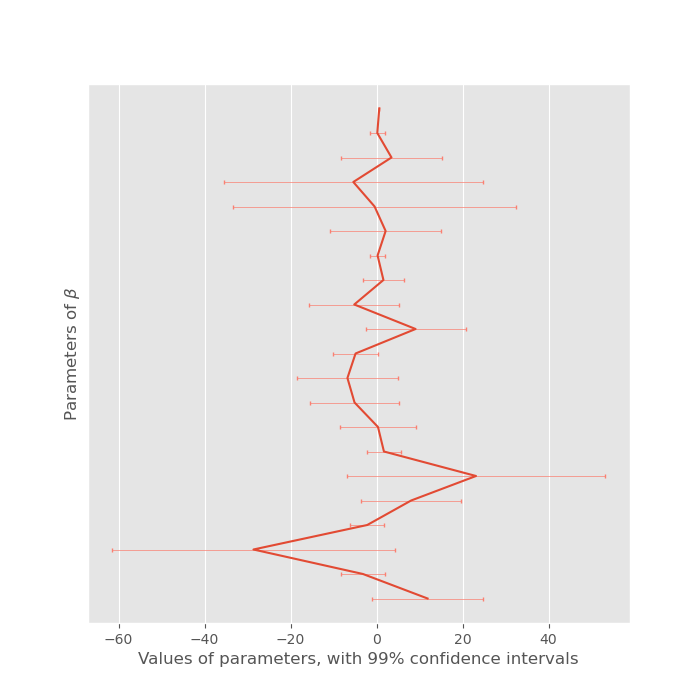
\includegraphics[width=0.5\textwidth]{../plots/conf_interval_beta_franke.png}
\end{center}
\caption{$99\%$ confidence interval for each $\beta$ parameter.}
\label{fig:conf_interval}
\end{figure}

\section{Resampling}

Next on the list of processes we want to verify works, is resampling. The data is scarce here, so resampling should give us better estimates of MSE, and also allow us to inspect the previously discussed bias-variance trade-off.

\subsection{Bias-variance trade-off}

Let us see if we can visualise thetrade-off with the data from the Franke function, and the bootstrap resampling technique. Our bootstrap function returns model variance and bias, as well as total mean squared error. We plot that data against different complexity scores, and look at it for ordinary linear regression, as well as for regularised Ridge and LASSO regression with a medium regularisation parameter $\lambda$. The results can be seen in fig \ref{fig:bias_variance_franke}.

\begin{figure}
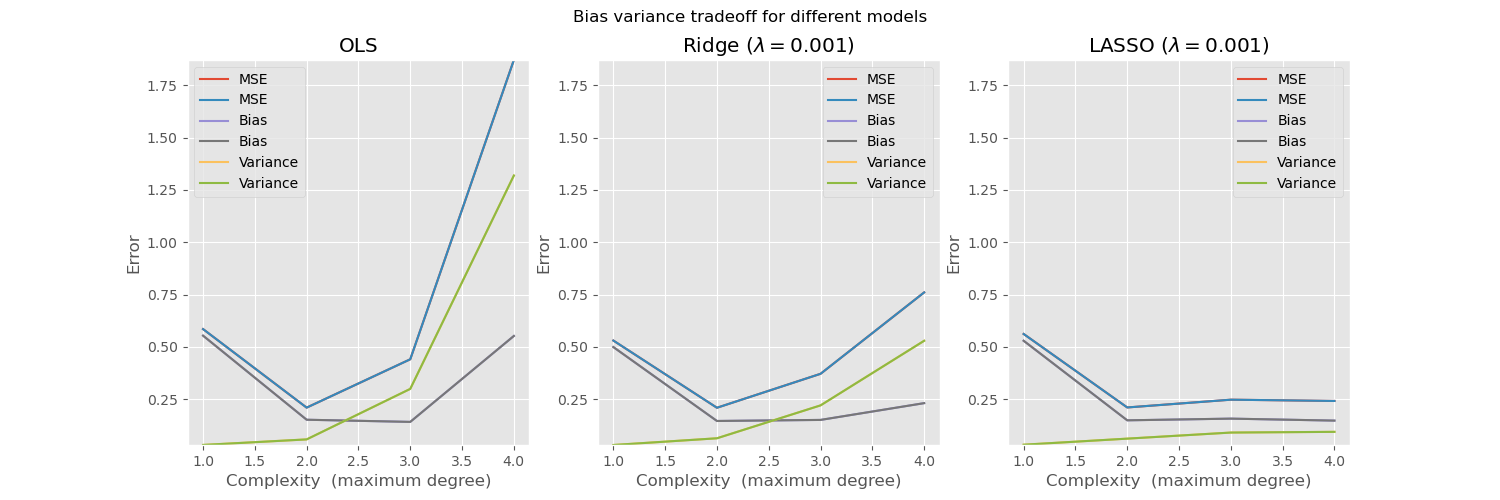
\includegraphics[width=\textwidth]{../plots/bias_variance_franke.png}
\caption{Bias, variance, and MSE estimated by bootstrap, for different models trained on the Franke dataset. There is a very strange issue with our code that makes the labels repeated, we're sorry for that.}
\label{fig:bias_variance_franke}
\end{figure}

If we start by examining the OLS plot, it shows that for low complexity, the bias is high but the variance is small. This makes sense because low degree polynomials have few degrees of freedom, so they can't really vary that much. Bias is big because they probably can't fit to the data that well either though. With some more complexity the bias and variance meet in the middle, before they both shoot up, with the variance growing quicker than the bias. Here, the models have a lot of options as to how to bend, and the way they bend is therefore highly dependent on which data it gets.

For the regularised plots, the tendencies is similar, but less extreme. The regularisation parameters keep the amount of overfitting down, and acts a lot more skeptical about believing the wild claims about the complex nature of the data than OLS does. LASSO does better than Ridge here, but this isn't enough data to conclude on anything, and we also haven't tested for different $\lambda$ values yet.

\subsection{Cross-validation}

Lastly, let us check that our k-fold cross-validation technique performs similarly to our already tested bootstrap method. If they don't, that's a good indication that something is wrong with one of them. We have therefore plotted errors for the same models as above, just with bootstrap and k-fold estimates of MSE.

\begin{figure}
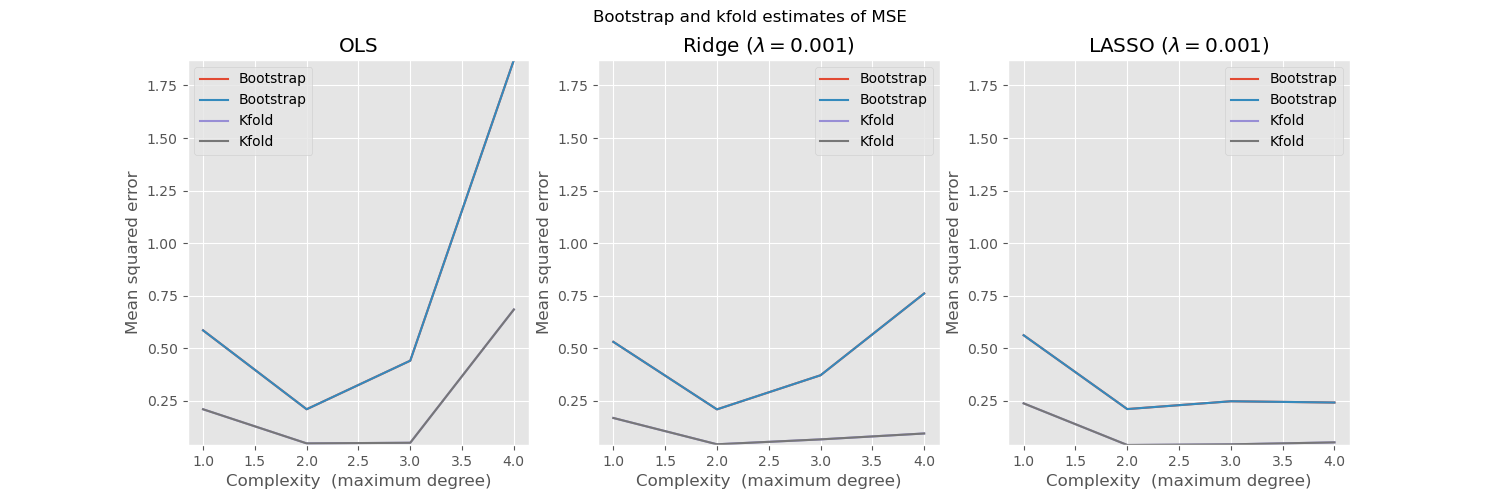
\includegraphics[width=\textwidth]{../plots/boot_kfold_franke.png}
\caption{MSE estimated by bootstrap and k-fold resampling techinques, for different models trained on the Franke dataset.}
\label{fig:boot_kfold_franke}
\end{figure}

\section{Results from tuning}

Now that all the individual parts have been tested, we are ready to try out the big Tune class, and see how well it is able to fit to the data. We won't be analysing it much, only explaining the methodology. In the next two chapters we'll look at the same results as the ones we're about to present, just for real terrain data, and we'll do that much more in depth.

\begin{figure}
\begin{center}
\caption{Hyperparameters tried out when tuning the models on the Franke function.\strut} 
\begin{tabular}{ l }
$p \in \{1, 2, \ldots, 15\} $ \strut \\
$\lambda_{Ridge} \in \{10^{i} \, | \, i \in \{-8, -7, -6, \ldots, 1\}\}$ \strut \\
$\lambda_{LASSO} \in \{10^{i} \, | \, i \in \{-24/16, -21/16, -18/16, -15/16, \ldots, 0\}\}$ \strut \\
\end{tabular}
\label{table:hyperparamters_franke}
\end{center}
\end{figure}

To explain our key plots, and discuss our methodology, but not use too much time on it, we are narrowing down this section to just cover the results from the bootstrap technique on the Ridge model. In fig \ref{fig:grid_ridge_kfold_franke} is a visualisation of the errors k-fold estimated during the validation phase, for different set of hyperparameters. In table \ref{table:optimal_models_franke} are the optimal parameters for each model estimated by the different techniques, with average just being the average of k-fold and bootstrap. Which model is optimal is just selected by the single lowest estimated MSE. One of the weaknesses with this is that the variance for estimation is now an important contributor to deciding which model is best. As seen in the grid search figure, there are many parameter-sets with very similar error metrics, so which one of them is the lowest is highly dependent on chance. A better way to do this would be to test out the candidates with the lowest errors some more times, and also test out the neighbouring region with a finer selection of parameter values, perhaps even using gradient decent methods. This would reduce variance, and also allow us to fine-tune the model the places where we are likely to find a good one, and not use the same parameter resolution everywhere. Perhaps a meta-reinforcement learning algorithm could do this well.

\begin{figure}
\includegraphics[width=\textwidth]{"../plots/franke_gridsearch_Ridge_Boot MSE".png}
\caption{Bootstrap grid search for best $\lambda$ and polynomial hyperparameters for the Ridge model, on the franke data. Complexity is lowest in the bottom left, and highest top right.}
\label{fig:grid_ridge_kfold_franke}
\end{figure}

\begin{figure}
\begin{center}
\caption{Optimal models as estimated by k-fold, bootstrap, and the average of them. In the rightmost column is the mean squared error of the model with those paramaters trained on the training set, and tested once on the testing set.} 
\begin{tabular}{llllll}
\toprule
    &         &    Lambda & Poly & Validation &      Test \\
Model & Resampling technique &           &      &            &           \\
\midrule
\multirow{3}{*}{Ridge} & Bootstrap & 1.000e-03 &   11 &  1.721e-01 & 4.525e-02 \\
    & Kfold & 1.000e-02 &    1 &  4.652e-02 & 6.325e-02 \\
    & Average & 1.000e-03 &   11 &  1.135e-01 & 4.525e-02 \\
\cline{1-6}
\multirow{3}{*}{Lasso} & Bootstrap & 1.389e-01 &    3 &  1.361e-01 & 1.131e-01 \\
    & Kfold & 3.162e-02 &   10 &  4.944e-02 & 6.522e-02 \\
    & Average & 8.483e-02 &   12 &  1.097e-01 & 8.316e-02 \\
\cline{1-6}
\multirow{3}{*}{OLS} & Bootstrap & 0.000e+00 &    4 &  1.826e-01 & 4.675e-02 \\
    & Kfold & 0.000e+00 &    1 &  4.842e-02 & 6.325e-02 \\
    & Average & 0.000e+00 &    4 &  1.168e-01 & 4.675e-02 \\
\bottomrule
\end{tabular}
.
\label{table:optimal_models_franke}
\end{center}
\end{figure}

In fig \ref{fig:ridge_bootstrap_best} is the model the bootstrap deemed optimal, tested on the testing set. Visually, the model looks like a good fit to the underlying structure, even though it seems as if a polynomial of higher degree should be able to capture the smaller peak in the middle of the plot as well.

\begin{figure}
\includegraphics[width=\textwidth]{"../plots/franke_test_Ridge_p11_lambda0001".png}
\caption{Terrain predicted on franke function testing data by Ridge with $\lambda = 10^{-8}$ and with maximum degree of $3$. These parameters are suggested by bootstrap as the best model.}
\label{fig:ridge_bootstrap_best}
\end{figure}


\chapter{Results on real terrain data}

When using the tuning class discussed in the previous chapter, with the same parameters as we tried on the Franke function (table \ref{table:hyperparamters_franke}), these are the results that we get on our real terrain data.

\begin{figure}
\includegraphics[width=\textwidth]{"../plots/real_gridsearch_Ridge_Kfold MSE".png}
\caption{K-fold grid search for best $\lambda$ and polynomial hyperparameters for the Ridge model, on the real terrain data.}
\label{fig:grid_ridge_kfold_real}
\end{figure}

\begin{figure}
\includegraphics[width=\textwidth]{"../plots/real_gridsearch_Ridge_Boot MSE".png}
\caption{K-fold grid search for best $\lambda$ and polynomial hyperparameters for the LASSO model, on the real terrain data.}
\label{fig:grid_ridge_boot_real}
\end{figure}

\begin{figure}
\begin{center}
\caption{Optimal models as estimated by k-fold, bootstrap, and the average of them. In the rightmost column is the mean squared error of the model with those paramaters trained on the training set, and tested once on the testing set.} 
\begin{tabular}{llllll}
\toprule
    &         &    Lambda & Poly & Validation &      Test \\
Model & Resampling technique &           &      &            &           \\
\midrule
\multirow{3}{*}{Ridge} & Bootstrap & 1.000e-08 &    4 &  3.406e+03 & 6.434e+02 \\
    & Kfold & 1.000e-07 &    7 &  5.984e+01 & 4.358e+02 \\
    & Average & 1.000e-03 &    8 &  1.753e+03 & 4.164e+02 \\
\cline{1-6}
\multirow{3}{*}{Lasso} & Bootstrap & 3.162e-02 &    6 &  3.911e+03 & 5.562e+02 \\
    & Kfold & 3.162e-02 &   14 &  8.845e+01 & 5.519e+02 \\
    & Average & 3.162e-02 &    6 &  2.038e+03 & 5.562e+02 \\
\cline{1-6}
\multirow{3}{*}{OLS} & Bootstrap & 0.000e+00 &    4 &  3.437e+03 & 6.434e+02 \\
    & Kfold & 0.000e+00 &    7 &  5.935e+01 & 4.545e+02 \\
    & Average & 0.000e+00 &    4 &  1.790e+03 & 6.434e+02 \\
\bottomrule
\end{tabular}
.
\label{table:optimal_models_real}
\end{center}
\end{figure}

As demonstrated by both fig \ref{fig:grid_ridge_kfold_real}, fig \ref{fig:grid_ridge_boot_real}, and table \ref{table:optimal_models_real}, the real data encourages slightly lower polynomial degrees, but roughly the same $\lambda$ values as the Franke function generated data did. This would however look different for a different dataset with real terrain data, and isn't inherent to real vs synthetic data.

Something that is also even more visible here than on the Franke data, is how different the estimates for error are between bootstrap and k-fold. Most of the time, they mark out the same regions of parameter sets as relatively good or bad, but give estimates of how erronous models with those parameters are a magnitude apart. This can probably be attributed mostly to the different data they are getting trained on. While each bootstrap sample only contains a subset of the training set, out k-fold function makes it so that almost all the training and validation data is available for each model. The different amounts of data explains the k-fold estimated errors tendency to be lower. The fact that our k-fold estimate is based on data the bootstrap trained models are only evaluated on, likely explains the other discrepancies. See \path{/plots/animations/franke_tune_Lasso_bootstrapKfold.mp4} for an example of very different k-fold and bootstrap estimates.

Another difference between our resampling techniques is that k-fold seems to have a higher variance. The values seem to follow much less of a continous function, with our heatmaps showing single parameter sets with completely different error estimates than the ones around. We have already hypothesised that (our implementation of) k-fold should have a higher variance than bootstrap with our implementation, so this strengthens that hypothesis.

Comparing the test scores for for different model architectures, with the hyperparameters selected with the average of the bootstrap and the k-fold validation data, Ridge does the best here. LASSO comes a bit further behind, followed by OLS. LASSO might be at a disadvantage her because it seems as if lower $\lambda$ values benefitted it a lot, but we struggled with getting it to converge when we used $\lambda \in [\leftarrow, 10^-2]$.

\begin{figure}
\includegraphics[width=\textwidth]{"../plots/real_test_Ridge_p7_lambda1e-07".png}
\caption{Terrain predicted on real terrain testing data by ridge with $\lambda = 10^{-3}$ and with maximum degree of $8$. These parameters are suggested by k-fold as the best model.}
\label{fig:ridge_kfold_best_real}
\end{figure}

\section{Validation error vs test error}

The hyperparameter optimimisation procedure established seems to works well. It is able to find hyperparameters $\lambda$ and max degree for both Franke function generated data, and one example of real terrain data, that makes polynomials fit the data. However, we have so far only looked at the models it deemed best, and have not looked at the ones it discarded. It very well might be that these models are just above average, and that random hyperparameters can do almost as well on unseen data. To discuss this, we need to look at the relation between the validation mean squared errors of our bootstrap and k-fold functions, and mean squared error on test data. Plotting this for the Franke function, we get fig \ref{fig:test_validation_error_franke} for the Franke function data, and fig \ref{fig:test_validation_error_real} for the real terrain data. Please note that we have 160 000 datapoints in total, but that because we used $x_{sparsity} = 20$, only 800 of those were used in training and validation. The test errors are therefore expected to be a very good estimate of the actual error.

\begin{figure}
\begin{center}
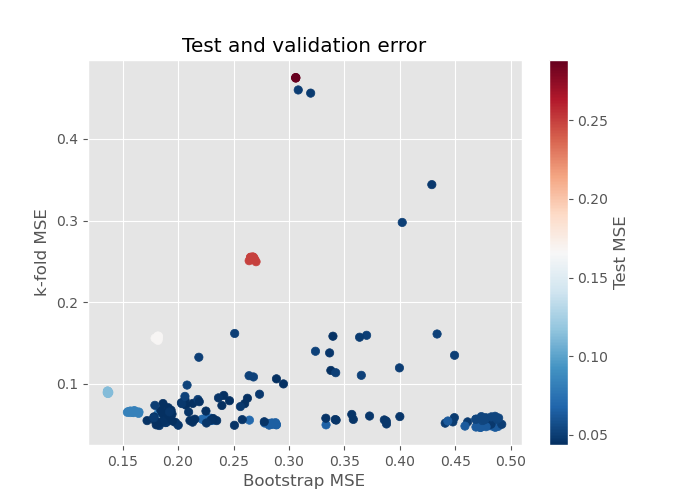
\includegraphics[width=0.8\textwidth]{../plots/test_validation_error_franke.png}
\end{center}
\caption{Franke terrain data: Validation errors calculated through resampling, with the colour of the points indicating their respective test error. Note that we have removed some outlier values.}
\label{fig:test_validation_error_franke}
\end{figure}

\begin{figure}
\begin{center}
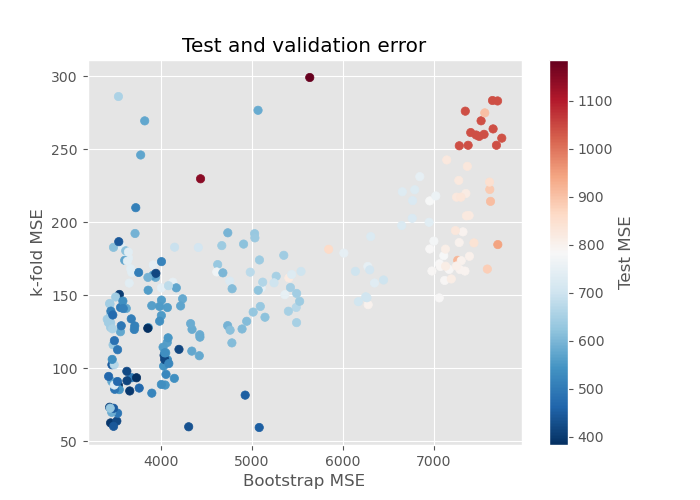
\includegraphics[width=0.8\textwidth]{../plots/test_validation_error_real.png}
\end{center}
\caption{Real terrain data: Validation errors calculated through resampling, with the colour of the points indicating their respective test error. Note that we have removed some outlier values.}
\label{fig:test_validation_error_real}
\end{figure}

The figures look quite different. While as the Franke function validation errors seem to poorly represent the test errors, the tuning for models on real terrain data fits pretty well. In the latter, most of the points are in the diagonal line going from little validation error with both resampling methods to high validation error with both, and in this series the test errors seem  to verify that they were mostly correct. There are points outside of this main series, where either k-fold or bootstrap has seen a structure the other one hasn't. Trying to fit a linear regression model to this data has noe been succesful, but we have little data.

The reason for the poorer performance on the Franke function data is likely because this data is very noisy, and therefore difficult to fit to. There is naturally a high variance between models.

All in all, it seems as if our validation is useful in predicting which models will do good, but far from perfect. After seeing this data, it is also hard to justify going back and changing the validation code, as that would make the test data less unseen, and risk having us fitting the models to it implicitly.

\chapter{Conclusions}

The implementation done here of linear regression is able to fit to terrain data, both synthetic and actual, well. Resampling techniques allows a decent idea of how a model would perform on unseen data, without requiring much data itself. With this validation procedure, the tuning class is able to pick out models that perform well, that don't overfit, but that also have a sufficient complexity. This is also due to regularisation techniques that discourage fitting to weak structures, which the difference between OLS and regularised linear regression here shows often to be false structures. The best model architecture for the data we've tested here has consistently been Ridge, with LASSO performing second best on the real terrain data, and OLS on the Franke function data.

Further work could look into a better tuning class that didn't use the same resolution everywhere, but explored areas of low validation errors further, resampling them more and trying out neighbouring hyperparameters.

It would also be interesting looking further into the relationship between test and validation error. Both looking at how much is really gained by resampling, which we have not discussed here, and seeing how well this implementation can predict test error for other datasets.

\chapter{Referencing}

T. Hastie, R. Tibshirani, and J. Friedman. \textit{The Elements of Statistical Learning: Data Mining, Inference, and Prediction, Second Edition.} Springer Series in Statistics. Springer New York, 2009. ISBN: 9780387848587.

Hjorth-Jensen, M. \textit{Lecture notes, FYS-STK3155} 2020.

\end{document}











































